%%%%%%%%%%%%%%%%%%%%%%%%%%%%%%%%%%%%%%%%%
% Thin Sectioned Essay
% LaTeX Template
% Version 1.0 (3/8/13)
%
% This template has been downloaded from:
% http://www.LaTeXTemplates.com
%
% Original Author:
% Nicolas Diaz (nsdiaz@uc.cl) with extensive modifications by:
% Vel (vel@latextemplates.com)
%
% License:
% CC BY-NC-SA 3.0 (http://creativecommons.org/licenses/by-nc-sa/3.0/)
%
%%%%%%%%%%%%%%%%%%%%%%%%%%%%%%%%%%%%%%%%%

%----------------------------------------------------------------------------------------
%	PACKAGES AND OTHER DOCUMENT CONFIGURATIONS
%----------------------------------------------------------------------------------------

\documentclass[letterpaper,10pt]{article} % Font size (can be 10pt, 11pt or 12pt) and paper size (remove a4paper for US letter paper)
\usepackage{geometry}
\geometry{paperwidth=4in,margin=.1in,paperheight=40in}
\usepackage[protrusion=true,expansion=true]{microtype} % Better typography
\usepackage{graphicx} % Required for including pictures
\usepackage{caption}
\usepackage{subcaption}
\usepackage{wrapfig} % Allows in-line images
\usepackage{amsmath,amsthm}
\usepackage{thmtools}
\usepackage{mathpazo} % Use the Palatino font
\usepackage[T1]{fontenc} % Required for accented characters
\linespread{1.05} % Change line spacing here, Palatino benefits from a slight increase by default

\makeatletter
\newcommand{\pipe}{\;\middle\vert\;}
\newcommand{\condp}[2]{\Pr\left( #1 \pipe #2 \right)}
\newcommand{\pr}[1]{\Pr\left( #1 \right)}
\newcommand{\condpe}[2]{\frac{\pr{#1,#2}}{\pr{#2}}}
\newcommand{\condpb}[2]{\frac{\condp{#2}{#1}\pr{#1}}{\pr{#2}}}
\newcommand{\norm}[1]{\left|#1\right|}
\DeclareMathOperator*{\argmin}{arg\,min}
\DeclareMathOperator*{\argmax}{arg\,max}
%theorem styling
\declaretheorem{theorem} 
\declaretheoremstyle[%
spaceabove=-6pt,%
spacebelow=6pt,%
headfont=\normalfont\itshape,%
postheadspace=1em,%
qed=\qedsymbol,%
headpunct={}
]{mystyle} 
\declaretheorem[name={},style=mystyle,unnumbered,
]{Proof}

\newcommand{\prove}[1]{
\begin{Proof}
\begin{align*}
#1
\end{align*}
\end{Proof}
}

\renewcommand{\@listI}{\itemsep=0pt} % Reduce the space between items in the itemize and enumerate environments and the bibliography

\renewcommand{\maketitle}{ % Customize the title - do not edit title and author name here, see the TITLE block below
\begin{flushright} % Right align
{\LARGE\@title} % Increase the font size of the title

{\large\@author} % Author name
\\\@date % Date

\end{flushright}
}

%----------------------------------------------------------------------------------------
%	TITLE
%----------------------------------------------------------------------------------------

\title{\textbf{Assignment 1}\\ % Title
Machine Learning 10-701} % Subtitle

\author{\textsc{Arjun Menon} % Author
\\{\textit{Carnegie Mellon University}}} % Institution

%----------------------------------------------------------------------------------------

\begin{document}

\maketitle % Print the title section

\section{Probability Review [Ahmed]}

\subsection{Why just 2 variables? Let's go for 3}

\subsubsection{}\label{subsubsec:1}
From the law of conditional probability,

\prove{
\frac{\condp{A,B}{C}}{\condp{B}{C}} &= \frac{\pr{A,B,C}}{\pr{C}} \frac{\pr{C}}{\pr{B,C}}\\
                                    &= \frac{\pr{A,B,C}}{\pr{B,C}}\\
                                    &= \frac{\pr{A,D}}{\pr{D}}\\
                                    &= \condp{A}{D}\\
                                    &= \condp{A}{B,C} \qedhere
}

\subsubsection{}\label{subsubsec:2}
\prove{
\sum_{B}\condp{A,B}{C} &= \sum_{B}\condpe{A,B}{C}\\
&=\condpe{A}{C}\\
&=\condp{A}{C} \qedhere
}

\subsubsection{}
Using result from Problem~\ref{subsubsec:1} and Problem~\ref{subsubsec:2},
\prove{
\sum_{B}\condp{A}{B,C}\condp{B}{C} &= \sum_{B}\condp{A,B}{C}\\
&= \condp{A}{C} \qedhere
}

\subsection{Evaluating Test Results}

\subsubsection{}
The probability that a transation succeeds given that it was handled by $A2$ is
\begin{align*}
\condp{Success}{A=2} &= \condpe{Success}{A=2}\\
&= \frac{\norm{Success, A=2}}{\norm{A=2}}\\
&= \frac{2150}{2150+500}\\
&= 0.811
\end{align*}

\subsubsection{}
If we recommend $A2$ then we need to see that
\prove{
\condp{Success}{A=2} &\geq \condp{Success}{A=1}\\
0.811 &\geq \frac{6000}{6000+1700}\\
0.811 &\geq 0.779 \qedhere
}

\subsubsection{}
The statement about the probability of $A2$ handling a transaction successfully given $A1$ handled it successfully is given by,
\prove{
\condp{A2_{suc}}{A1_{suc}} &= \condpe{A2_{suc}}{A1_{suc}}\\
&\geq \frac{\pr{A2_{suc}}+\pr{A1_{suc}}-1}{\pr{A1_{suc}}}\\
&= \frac{\frac{2150}{2150+500}+\frac{6000}{6000+1700}-1}{\frac{6000}{6000+1700}}\\
&= 0.757 \\
\condp{A2_{suc}}{A1_{suc}} &\geq 0.757 \qedhere
}

\subsection{Monty Hall Problem}

Solving for $\pr{car3 \pipe open2, choose1}$ we get,
\begin{align*}
 &\pr{car3 \pipe open2, choose1} = \frac{\condp{car3, open2}{choose1}}{\condp{open2}{choose1}}\\
 &=\frac{\condp{open2}{choose1,car3}\condp{car3}{choose1}}{\condp{open2}{choose1}} \\
 &=\frac{1 \times \tfrac{1}{3}}{\tfrac{1}{2}} \\
 &=\tfrac{2}{3}
\end{align*}


and solving for $\pr{car1 \pipe open2, choose1}$ we get,
\begin{align*}
 &\pr{car1 \pipe open2, choose1} = \frac{\condp{car1, open2}{choose1}}{\condp{open2}{choose1}}\\
 &=\frac{\condp{open2}{choose1,car1}\condp{car1}{choose1}}{\condp{open2}{choose1}} \\
 &=\frac{\tfrac{1}{2} \times \tfrac{1}{3}}{\tfrac{1}{2}} \\
 &=\tfrac{1}{3}
\end{align*}

which gives us,

\prove{
  \frac{\pr{car3 \pipe open2, choose1}}{\pr{car1 \pipe open2, choose1}} &= \frac{\tfrac{2}{3}}{\tfrac{1}{3}} \\
  &= 2 \qedhere
}

\newpage
\section{Regression [Leila]}
\subsection{Linear Regression}
Starting with the definition of the MLE estimate,

\begin{align*}
\beta_{MLE} &= \argmax_{\beta \in B} \condp{Data}{\beta}\\
&= \argmax_{\beta \in B} \prod_{i=1}^n \condp{y_i}{x_i, \beta}\\
&= \argmax_{\beta \in B} \prod_{i=1}^n \left(\frac{1}{\sqrt{2\pi\sigma^2}}\right) \exp\left( \frac{-1}{2\sigma^2} (y_i-\beta x_i)^2 \right) \\
&= \argmax_{\beta \in B} \left(\frac{1}{\sqrt{2\pi\sigma^2}}\right)^n \exp\left( \frac{-1}{2\sigma^2} \sum_{i=1}^n (y_i-\beta x_i)^2 \right) \\
&= \argmax_{\beta \in B} \left(\frac{1}{\sqrt{2\pi\sigma^2}}\right)^n \exp\left( \frac{-1}{2\sigma^2} (Y-X\beta)^T(Y-X\beta) \right) \\
\end{align*}

The expressions above is maximized when $(Y-X\beta)^T(Y-X\beta)$ is minimized where,

\begin{align*}
Y &= \left[ \begin{array}{c}
y_1 \\
\vdots \\
y_n \end{array} \right] \\
X &= \left[ \begin{array}{c}
x_1^T \\
\vdots \\
x_n^T \end{array} \right]
\end{align*}

Minimizing $L=(Y-X\beta)^T(Y-X\beta)$ by taking the gradient with respect to $\beta$, setting to zero, and solving for $\beta$ gives us the $\beta_{MLE}$ as follows,

\prove{
L &= (Y-X\beta)^T(Y-X\beta) \\
L &= Y^TY -2Y^TX\beta+\beta^TX^TX\beta \\
\nabla_{\beta}L &= 0 - 2Y^TX + (X^TX +(X^TX)^T)\beta \\
0 &= -2Y^TX+2X^TX\beta \\
X^TX\beta &= X^TY \\
\beta_{MLE} &= (X^TX)^{-1}X^TY\qedhere
}

\subsection{Ridge Regression}

Starting with the definition of the MAP estimate,

\begin{align*}
&\beta_{MAP} = \argmax_{\beta \in B} \condp{\beta}{Data}\\
&= \argmax_{\beta \in B} \condpb{\beta}{Data}\\
&\propto \argmax_{\beta \in B} \condp{Data}{\beta}\pr{\beta}\\
&= \argmax_{\beta \in B} \left[ \prod_{i=1}^n \condp{y_i}{x_i, \beta}\right] \pr{\beta}\\
&= \argmax_{\beta \in B} \left[ \prod_{i=1}^n \frac{1}{\sqrt{2\pi\sigma^2}} \exp\left( \frac{-1}{2\sigma^2} (y_i-\beta x_i)^2 \right) \right] \exp\left(\frac{-\beta^T\beta}{2\lambda^2}\right)\\
&\propto \argmax_{\beta \in B} \left[ \exp\left( \frac{-1}{2\sigma^2} \sum_{i=1}^n (y_i-\beta x_i)^2 \right) \right] \exp\left(\frac{-\beta^T\beta}{2\lambda^2}\right)\\
&= \argmax_{\beta \in B} \left[ \exp\left( \frac{-1}{2\sigma^2} (Y-X\beta)^T(Y-X\beta) \right) \right] \exp\left(\frac{-\beta^T\beta}{2\lambda^2}\right)\\
&= \argmax_{\beta \in B} \exp\left( \frac{-1}{2\sigma^2} (Y-X\beta)^T(Y-X\beta) + \frac{-\beta^T\beta}{2\lambda^2}\right)\\
\end{align*}

The expressions above is maximized when $\frac{-1}{2\sigma^2}(Y-X\beta)^T(Y-X\beta)-\frac{\beta^T\beta}{2\lambda^2}$ is minimized where,

\begin{align*}
Y &= \left[ \begin{array}{c}
y_1 \\
\vdots \\
y_n \end{array} \right] \\
X &= \left[ \begin{array}{c}
x_1^T \\
\vdots \\
x_n^T \end{array} \right]
\end{align*}

Since $\sigma=1$, we can also get rid of the 2's and minimize $L=(Y-X\beta)^T(Y-X\beta)-\frac{\beta^T\beta}{\lambda^2}$ by taking the gradient with respect to $\beta$, setting to zero, and solving for $\beta$ gives us the $\beta_{MAP}$ as follows,

\prove{
L &= (Y-X\beta)^T(Y-X\beta)-\frac{\beta^T\beta}{\lambda^2}\\
L &= Y^TY -2Y^TX\beta+\beta^TX^TX\beta-\lambda^\prime\beta^T\beta \\
\nabla_{\beta}L &= 0 - 2Y^TX + (X^TX +(X^TX)^T)\beta -2\lambda^\prime\beta \\
0 &= -2Y^TX+2X^TX\beta-2\lambda^\prime\beta \\
(X^TX+\lambda^\prime)\beta &= X^TY \\
\beta_{MAP} &= (X^TX+\lambda^\prime)^{-1}X^TY\qedhere
}


\newpage
\section{Classification [Dougal]}
\subsection{Drawing decision boundaries}

\begin{figure}[h]
\centering
\begin{subfigure}[b]{\textwidth}
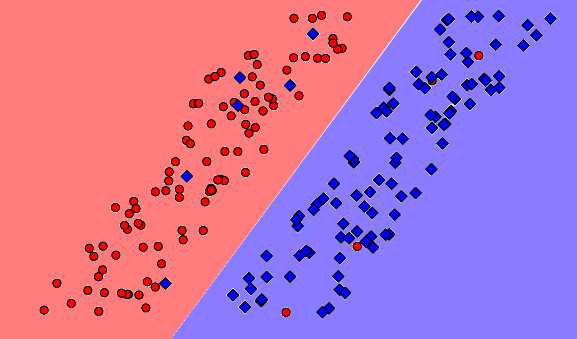
\includegraphics[width=\textwidth]{handout/q3-1-logistic}
\caption{Logistic Regressor decision boundary}
\label{fig:log1}
\end{subfigure}%

\begin{subfigure}[b]{\textwidth}
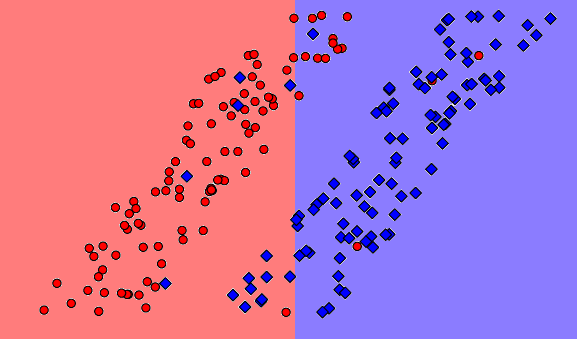
\includegraphics[width=\textwidth]{handout/q3-1-bayes}
\caption{Naive Bayes decision boundary}
\label{fig:bayes1}
\end{subfigure}

\begin{subfigure}[b]{\textwidth}
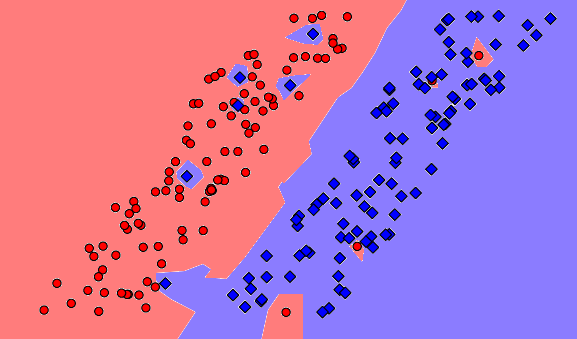
\includegraphics[width=\textwidth]{handout/q3-1-NN}
\caption{1-NN decision boundary}
\label{fig:1nn1}
\end{subfigure}

\begin{subfigure}[b]{\textwidth}
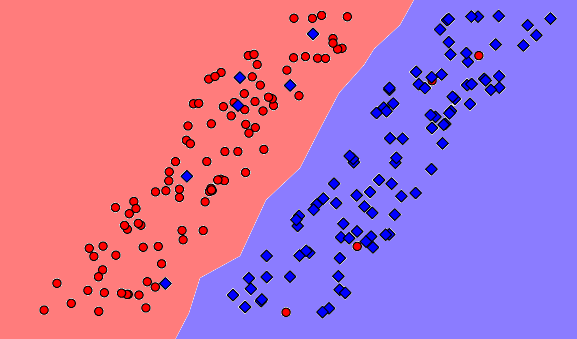
\includegraphics[width=\textwidth]{handout/q3-1-10NN}
\caption{10-NN decision boundary}
\label{fig:10nn1}
\end{subfigure}

\caption{Decision boundaries of the first data set}\label{fig:decision1}
\end{figure}

In Figure~\ref{fig:decision1} we can see the decision boundaries on the first data set. 

Figure~\ref{fig:log1} shows the logistic regression boundary which liear between the two sets. 

Figure~\ref{fig:bayes1} shows that Naive Bayes performs poorly on this data set because the features are NOT independant of each other. One feature becomes completely irrelevant to classification.

Figure~\ref{fig:1nn1} shows that 1-NN is very sensitive to the noise, and creates strange voronoi regions where it provides the obviously wrong label.

Figure~\ref{fig:10nn1} shows 10-NN performing very well on noise, and providing a boundary similar to the logistic regressor.

\begin{figure}[h]
\centering
\begin{subfigure}[b]{\textwidth}
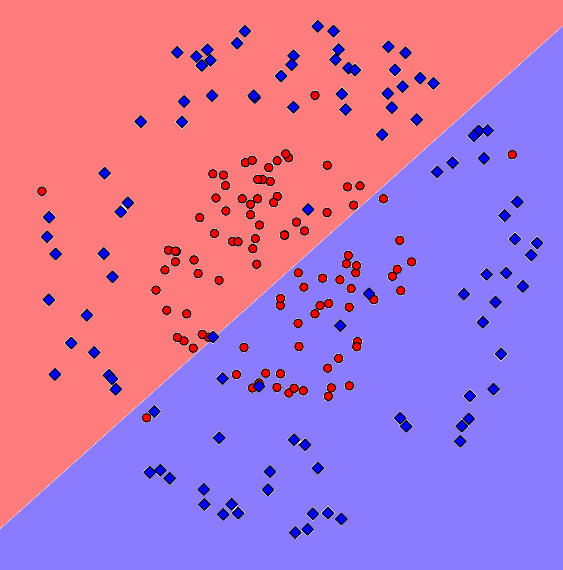
\includegraphics[width=\textwidth]{handout/q3-2-logistic}
\caption{Logistic Regressor decision boundary}
\label{fig:log2}
\end{subfigure}%

\begin{subfigure}[b]{\textwidth}
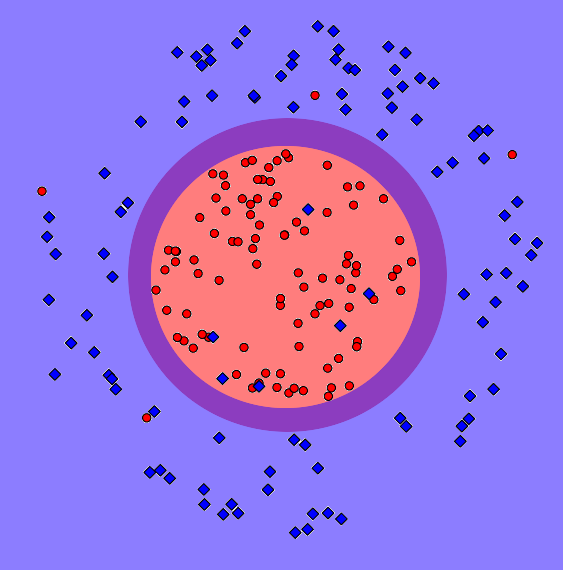
\includegraphics[width=\textwidth]{handout/q3-2-bayes}
\caption{Naive Bayes decision boundary}
\label{fig:bayes2}
\end{subfigure}

\begin{subfigure}[b]{\textwidth}
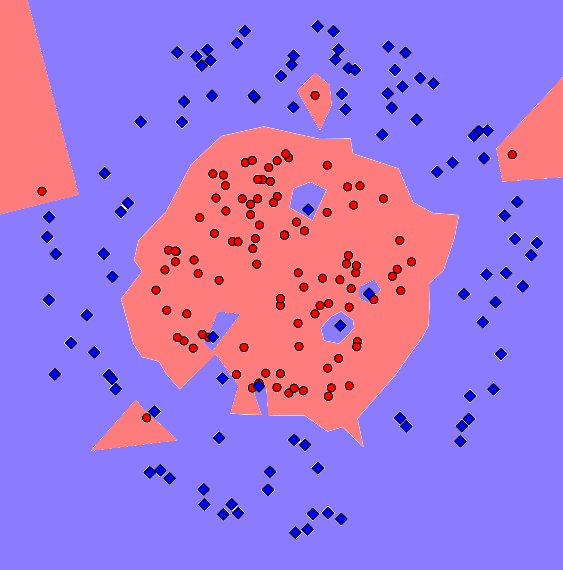
\includegraphics[width=\textwidth]{handout/q3-2-NN}
\caption{1-NN decision boundary}
\label{fig:1nn2}
\end{subfigure}

\begin{subfigure}[b]{\textwidth}
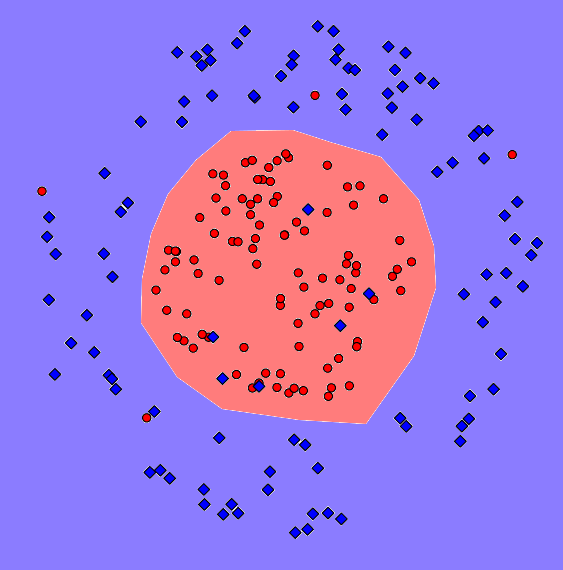
\includegraphics[width=\textwidth]{handout/q3-2-10NN}
\caption{10-NN decision boundary}
\label{fig:10nn2}
\end{subfigure}

\caption{Decision boundaries of the second data set}\label{fig:decision2}
\end{figure}

Figure~\ref{fig:decision2} shows the classifier decision boundaries on the circular data set.

Figure~\ref{fig:log2} shows the logistic regression decision boundary. Note that it is unable to find a line to seperate the data. It performs poorly on this data set.

Figure~\ref{fig:bayes2} shows the Naive Bayes classifier decision boundary creating roughly circular decision boundary. This is because the guassian for the red-data on both features are highly kurtotic so for when posterior probability for red is high are represented by a roughly circular region.

Figure~\ref{fig:1nn2} shows the 1-NN classifier decision boundary. You can see that the same sensitivity to noise occurs, and huge voronoi regision of red appear on the peripherry.

Figure~\ref{fig:10nn2} shows the 10-NN classifier decision boundary which is robust to noise and has no patches like in 1-NN.

\subsection{Defeating classifiers}

%------------------------------------------------
%\bibliographystyle{unsrt}
%\bibliography{sample}

%----------------------------------------------------------------------------------------

\end{document}
